\newpage
\mysection{Introduction \label{sec:crypthints}}

 This course is called "Advanced Structures and Algorithms" and its essence is learning how to create complex structures along with the algorithms that provide efficient ways to store and retrieve data from within those structures. The Efficiency of an advanced structure is something you will learn to measure by evaluating the \ccb{run times} (aka costs) of each algorithm we explore, and how the data structure used for storing the data may impact overall efficiency.\\
 
 In my opinion, this course is your first "real" programming course. Some students feel that data structures (1063) was a tough course, and I don't disagree, however this course will require you to use all the skills you gained ... and then some. If you struggle with arrays, pointers, or linked lists you may want to come see me, or review the following materials:
 
 \begin{enumerate}
    \item \href{https://cs.msutexas.edu/~griffin/materials/Arrays.pdf}{Arrays}
    \item \href{https://cs.msutexas.edu/~griffin/materials/PointersAndMemory.pdf}{Pointers and Memory}
    \item \href{https://cs.msutexas.edu/~griffin/materials/LinkedListBasics.pdf}{Linked List Basics}
\end{enumerate}

\mysubsection{Array vs List}

I just eluded to the fact that your previous course had a goal of getting you comfortable with certain concepts. One of those concepts was: "Do I use an array to store my data? Or do I used a linked list?"  In computer science we use the terms: \ccb{array based structure} and \ccb{list based structure} for our two choices on how to store data in memory. However, to create list based structures you need to "link" memory locations, and so you were introduced to \ccb{pointers} which allowed you to create \ccb{linked lists}. Both arrays and linked lists have pros and cons associated with them, and understanding the pros and cons of each structure will help you understand why certain algorithms work better when implemented using one or the other. There is not a single best choice, an array can do anything a linked list can, and vice versa. But in certain situations, one will be better than the other. This course will help you know when to choose one over the other. Below is a summary of both: \\

\ccb{Array:}\\
\vspace{-.5cm}
\begin{enumerate}
    \item Direct access (random access) using subscript.
    \item Growing and shrinking is costly.
    \item Bad for lots of insertions and deletions (because of empty slots and need for shifting).
    \item Good for searching (if items are ordered).
\end{enumerate}

\ccb{Linked Lists: }\\
\vspace{-.5cm}
\begin{enumerate}
    \item Access requires traversal using a pointer.
    \item Grows and shrinks easily.
    \item Good for lots of insertions and deletions (because of previous point).
    \item Bad for searching (linear only).
\end{enumerate}

\begin{center}
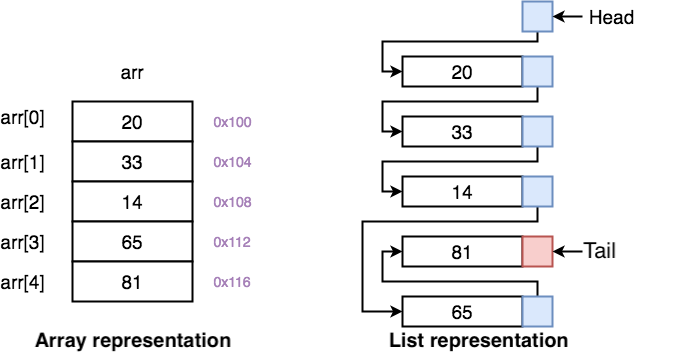
\includegraphics[scale=.35]{images/array-vs-linked-list.png}
\end{center}

\begin{table}[ht]
\footnotesize
    \centering
    \begin{tabular}{|p{3cm}|p{5.5cm}|p{6cm}|}
        \hline
        \textbf{Comparison} & \textbf{Array} & \textbf{Linked List} \\
        \hline
        Generic & Contiguous memory locations of fixed size.& Dynamically allocated memory locations linked by pointers. \\
        \hline
        Size & Fixed at allocation. & Grows and shrinks easily. \\
        \hline
        Order of the elements &	Stored consecutively & Stored randomly\\
        \hline
        Accessing  & Direct access using subscript. & Sequentially accessed from head or other pointer. \\
        \hline
        Insertion and deletion & Slow if shifting is required. & Easier, fast and efficient.\\
        \hline
        Searching &	Binary search (if ordered values) and linear search. & Linear search only.\\
        \hline
        Memory required & Size of data stored.	& Size of data stored + pointer.\\
        \hline
    \end{tabular}
    \caption{Array VS Linked List\supcite{arrayvlinked}}
    \label{table:listvarray}
\end{table}

\mysubsection{Stacks and Queues}

Something else you should have taken away from your previous CS course is the concepts of two simple data structures: 1) \ccb{Stacks} and 2) \ccb{Queues}. Not only the concept of how they work (LIFO v FIFO), but also how to implement either of them using an array or a list.

 \begin{enumerate}
    \item \href{https://cs.msutexas.edu/~griffin/materials/StacksAndQueues.pdf}{Stacks and Queues Helper Material}
\end{enumerate}

There are many other things you should have taken away from your data structures course, but to continue in this class with some comfort, you really should comfortably grasp the following. Each of the items is a link to a gist with example code. 

 \begin{enumerate}
    \item \href{https://gist.github.com/rugbyprof/1ebeeb6a5942050b8e326762f114cddd}{Array Based Stack}
    \item \href{https://gist.github.com/rugbyprof/84fd677220eeae40bdc7be07600f6f58}{List Based Stack}
    \item \href{https://gist.github.com/rugbyprof/3960ce651ae5397f525b1d83a69fa899}{Array Based Queue}
    \item \href{https://gist.github.com/rugbyprof/cb9bb1627d234e0987369028da524197}{List Based Queue}
\end{enumerate}

If you can comfortably write all of those combinations basically from scratch, you are in a good position to continue. If not, practice!! 

\mysubsection{Algorithm vs Data Structure}

We have laid the groundwork and are ready to discuss what \textit{advanced structures \& algorithms} really are. They are (to put it another way) \textit{advanced \underline{data} structures \textbf{and the} algorithms \underline{used to} \underline{manipulate them}}. They are two separate concepts, but in this context they are highly related. Lets look at each term separately.\\

\textbf{Data Structure:} In computer science, a \textit{data structure} is a data organization, management, and storage format that enables efficient access and modification. More precisely, a data structure is a collection of data values, the relationships among them, and the functions or operations that can be applied to the data\supcite{wiki:ds}.\\

\textbf{Algorithm:} In mathematics and computer science, an \textit{algorithm}  is a finite sequence of well-defined, computer-implementable instructions, typically to solve a class of problems or to perform a computation. Algorithms are always unambiguous and are used as specifications for performing calculations, data processing, automated reasoning, and other tasks\supcite{wiki:alg}.\\ 

Both of these fundamental blocks are needed to solve problems in computer science, and are also why our field is so tightly coupled with mathematics. A good data structure allows for the efficient storage and retrieval of data. But to make this happen we (typically) need to follow a sequence of well-defined instructions to guarantee \textit{unambiguous} behavior by our data structure \footnote{Describe what "ambiguous" behavior of an algorithm or data structure might be}. What exactly does that mean? Let's use an example to clarify.\\

\mysubsection{Stack vs Queue Example}

Let me explain how the two relate by providing an example using concepts you have already been introduced to. When implementing a data structure, you have two choices for your \ccb{storage format}: 1) Array Based or 2) a List Based structure\footnote{Or some hybrid of the two. But in general, those are the choices}. In other words I can use an \ccb{array} or I can use a \ccb{linked list} to implement my stack or queue. But what exactly makes an array or a linked list a \ccb{stack} or a \ccb{queue}? They both have push operations. They both have pop operations\footnote{Some books use 'enqueue' and 'dequeue' as operations for a queue, but they still add and remove items.}. The difference is in the algorithm that you employ to add or retrieve that data. A stack uses \ccb{LIFO} (Last In First Out) while a queue uses \ccb{FIFO} (First In First Out). A small change in the algorithm you use to implement the data structure changes the entire behavior of that data structure regardless of the \textit{storage format} that you chose. The algorithm that we use to add or remove items from each structure will guarantee, unambiguously, that the data structure will behave in a correct manner. \\

Let's look at the difference in algorithms between a stack and a queue. This example will use an array as its storage container. See the implementation of \ccb{Push} and \ccb{Pop} below: \\

\begin{table}[H]
\begin{tabular}{|M{0.1\textwidth}|m{0.45\textwidth}|m{0.45\textwidth}|}
    \hline
    \textbf{Op} & \textbf{Stack} & \textbf{Queue} \\
    \hline
    
    \textbf{Push} 
    &
    \begin{minipage}[t]{0.5\textwidth}
    \begin{minted}[]{c++}
    //
    bool Push(int x){
        if(!full()){
            ++top;
            array[top] = x;
            return true;
        }
        return false;
    }
    \end{minted}
    \end{minipage}
    &
    \begin{minipage}[t]{0.5\textwidth}
    \begin{minted}[bgcolor=clear]{c++}
    bool Push(int x){
        if(!full()){
            array[rear] = x;
            rear = (rear + 1) % array_size;
            return true;
        }
        return false;
    }
    \end{minted}
    \end{minipage}\\
    \hline
    \textbf{Pop} 
    &
    \begin{minipage}[t]{0.5\textwidth}
    \begin{minted}[]{c++}
    //
    int Pop(){
        if(!empty()){
            int retval = array[top];
            --top;
            return retval;
        }
        return INT_MIN;
    }
    \end{minted}
    \end{minipage}
    &\begin{minipage}[t]{0.5\textwidth}
    \begin{minted}[bgcolor=clear]{c++}
    int Pop(){
        if(!empty()){
            int retval = array[front];
            front = (front + 1) % array_size;
            return retval;
        }
        return INT_MIN;
    }
    \end{minted}
    \end{minipage}\\
    \hline
\end{tabular}
\caption{Algorithms for Stack and Queue}
\label{table:stackvqueue}
\end{table}

If you notice, the methods used to implement \textit{Push} and \textit{Pop} for both a \textit{Stack} and a \textit{Queue} are nearly identical, however, one small change to the algorithm used to control where items get inserted or removed, changes the behavior in a pretty big way. It changes from \textit{FIFO} to \textit{LIFO} and vice versa depending on whether you insert and remove from "Top" or if your insert and remove from "Rear" and "Front" respectively. \\

Look at the example below of inserting values into each data structure using their respective algorithms. We tend to draw stacks with a vertical orientation, and queues with a horizontal orientation because those orientations fit visually with how most individuals picture each respective structure. A "stack" is pictured like items are being "stacked" one on top of another, and a "queue" is pictures like items "getting in line" one behind the other. 

\begin{longtable}{|M{2cm}|M{6cm}|M{6cm}|}
    \hline
    \textbf{OP} & \textbf{Stack} & \textbf{Queue} \\
    \hline
    & 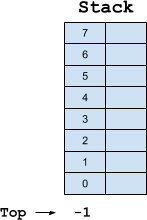
\includegraphics[scale=.35]{images/stack_intro_01.png} & 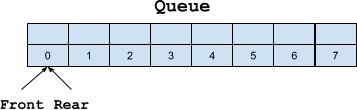
\includegraphics[scale=.35]{images/queue_intro_01.png}\\
    & \texttt{Initial State} & \texttt{Initial State} \\
    \hline
    \textbf{Push 7} & 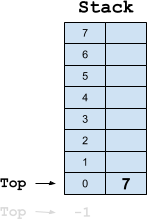
\includegraphics[scale=.35]{images/stack_intro_02.png} & 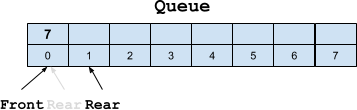
\includegraphics[scale=.35]{images/queue_intro_02.png} \\
    & 
    \begin{minipage}[l]{6cm}
    \texttt{1. Increment Top} \\
    \texttt{2. Insert item at Top}\\
    \end{minipage}
    & 
    \begin{minipage}[l]{6cm}
    \vspace{5mm}
    \texttt{1. Insert item at Rear} \\
    \texttt{2. Increment Rear}\\
    \end{minipage}\\
    \hline
    \textbf{Push 11} & 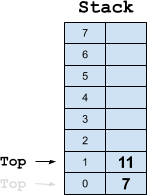
\includegraphics[scale=.35]{images/stack_intro_03.png} & 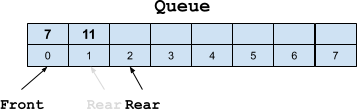
\includegraphics[scale=.35]{images/queue_intro_03.png} \\
    & 
    \begin{minipage}[l]{6cm}
    \texttt{1. Increment Top} \\
    \texttt{2. Insert item at Top}\\
    \end{minipage}\\
    & 
    \begin{minipage}[l]{6cm}
    \vspace{5mm}
    \texttt{1. Insert item at Rear} \\
    \texttt{2. Increment Rear}\\
    \end{minipage}\\
    \hline
    \textbf{Push 13,5,2}  & 
    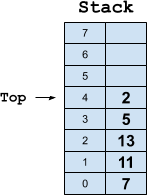
\includegraphics[scale=.35]{images/stack_intro_04.png} & 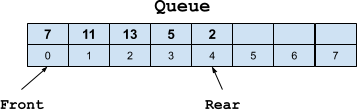
\includegraphics[scale=.35]{images/queue_intro_04.png} \\
    &
    \begin{minipage}[l]{6cm}
    \texttt{Resulting Stack After 13,5,2 are pushed} 
    \end{minipage}\\
    & 
    \begin{minipage}[l]{6cm}
    \vspace{5mm}
    \texttt{Resulting Queue After 13,5,2 are pushed} 
    \end{minipage}\\
    \hline 
    \caption{Stack Queue Example Inserts}
    \label{table:visible_stack_queue_add}
\end{longtable}

The resulting data structures are identical after inserting 5 values into each. The values are in the same order. They are using the same type of container (an array), and they have the same types of operations (Push, Pop). The main difference between the two is in how each algorithm implements the  "removal" method. Stacks remove from the "top" and queues remove from the "front", entirely changing the order in which they operate. But is that true? Below we remove an item from each, and yes, we get a 2 from the stack, and a 7 from the queue. But does the subtle differences in each algorithm make these structures really that different?

\begin{longtable}{|M{2cm}|M{6cm}|M{6cm}|}
    \hline
    \textbf{Pop} & 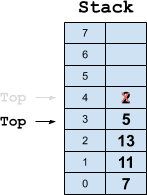
\includegraphics[scale=.35]{images/stack_intro_05.png} & 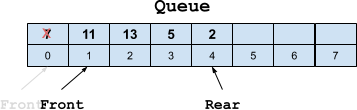
\includegraphics[scale=.35]{images/queue_intro_05.png} \\
    & 
    \begin{minipage}[l]{6cm}
    \texttt{1. Copy value at Top (2)} \\
    \texttt{2. Decrement Top}\\
    \texttt{3. Return value 2}\\
    \end{minipage}\\
    & 
    \begin{minipage}[l]{6cm}
    \vspace{5mm}
    \texttt{1. Copy value at Front (7)} \\
    \texttt{2. Increment Front}\\
    \texttt{3. Return value 7}\\
    \end{minipage}\\
    \hline 
    \textbf{Pop} & 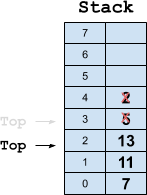
\includegraphics[scale=.35]{images/stack_intro_06.png} & 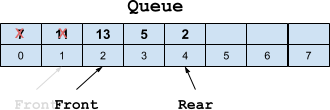
\includegraphics[scale=.35]{images/queue_intro_06.png} \\
    & 
    \begin{minipage}[l]{6cm}
    \texttt{1. Copy value at Top (5)} \\
    \texttt{2. Decrement Top}\\
    \texttt{3. Return value 5}\\
    \end{minipage}\\
    & 
    \begin{minipage}[l]{6cm}
    \vspace{5mm}
    \texttt{1. Copy value at Front (11)} \\
    \texttt{2. Increment Front}\\
    \texttt{3. Return value 11}\\
    \end{minipage}\\
    \hline 
    \caption{Stack Queue Example Removals}
    \label{table:visible_stack_queue_remove}
\end{longtable}

Try mixing up the operations performed by doing pushes and pops randomly\footnote{I didn't do this because I didn't want to have a 4 page example}. Our containers would have been extremely different in that scenario. In fact you should do this as an exercise to make sure you understand how both data structures work.\\

I hope that I have shown you that a "data structure" coupled with an "algorithm" become partners in creating "advanced structures". It is a little stretch to call a stack or a queue an "advanced structure", but as introductory examples, they work fine. They showed us that a "data structure" stores data and an "algorithm" unambiguously controlled how that data was stored. Now all we need to do is use more complex algorithms to control how data the data is stored and retrieved, and we will be solving cool complex problems\footnote{Also known as "Advanced Structures \& Algorithms"}.\\

\mysubsection{Course Content Overview}

Linear Data Structure: Linked List, Stack, Queue, Array.
Hierarchical data structures: Tree, Heap, Trie.
Other Data Structures: Hash, Graph, Matrix.

A data structure is a data organization, management, and storage format that enables efficient access and modification.
Most of the problems in computer science have some sort of data associated with, using which we have to solve the problem or we have to come up with a sort of conclusion.
So, as the above line states, the data structure is a way to organize and manage that data at memory level such that we can effectively and efficiently do operation on that data. Here, operations on data are like accessing, modifying or maybe deleting that data.
In other words, we have to structure and organize the raw data available for the problem statement, such that we can efficiently perform the required operation to solve the problem.
More precisely, a data structure is a collection of data values, the relationships among them, and the functions or operations that can be applied to the data.
Generally, developers know that Data structure is just an organization and management of data but it’s more than that and that’s why Wikipedia has added the above line in the definition. This statement is equally important to understand the role of data structure.
Here, in this statement the most useful words are “… the functions or operations that can be applied to the data”. If you don’t have much knowledge yet about actual data structures(Linked List, Stack, Queue, etc.), then it is very difficult to understand this line of definition.
In layman’s language, we can say that many data structures have the same organization of data at the memory level but they can provide the different functions and operations on them which differentiate with each other.
Let me give an example of the same. Stack and Queue can be implemented using Linked List have the same data organization at the memory level but they are providing different functions that are useful in different scenarios. Like, Queue can be used for First in first out(FIFO) scenarios while Stack can be used in Last in first out(LIFO) scenarios.
Few examples of Data Structures
Linear Data Structure: Linked List, Stack, Queue, Array.
Hierarchical data structures: Tree, Heap, Trie.
Other Data Structures: HashMap, Graph, Matrix.
Note: If you are a beginner and don’t know much about Queues or Stacks or LinkedList, don’t worry. You can follow me for my upcoming series on “Data Structures for beginners with the real-world application”.
Algorithms
An algorithm is a finite sequence of well-defined, computer-implementable instructions, typically to solve a class of problems or to perform a computation. Algorithms are unambiguous specifications for performing calculation, data processing, automated reasoning, and other tasks. - Wikipedia

I can understand that as a beginner you may be confused after reading this definition. Let’s understand this in layman’s language first and then jump to the technical definition of Algorithm.
In the simplest words, Algorithm is nothing but a sequence of steps to be followed to solve any problem or to achieve the desired output.
By taking this simplest definition now in your mind, let's understand the words mentioned in Wikipedia’s definition.
Finite sequence: The number of steps to solve a problem should be finite in numbers.
Well-defined: There should not be any ambiguity in any step.
Computer-implementable instructions: As we are talking about Computer Science related problems here, the steps should be understood by the computer.
A class of problems: Set of problems that have the same end goal or may have the same sequence of steps to reach the desired output.
Now let me put this down in one sentence.
An algorithm is a process of finite well-defined steps to be carried out to solve a particular class of problems or to get the desired output.
Few examples of Algorithms
Sorting Algorithms: Merge Sort, Quick Sort, Tim Sort, etc.
Searching Algorithms: Linear Search, Binary Search.
Shortest Path Algorithms: Dijkstra’s algorithm, Bellman-Ford algorithm.
Summing-up
Data Structure is about organising and managing data effectively such that we can perform specific operation efficiently, while Algorithm is a step-by-step procedure to be followed to reach the desired output.
To understand the Data Structure in a meaningful way, you also have to consider the understanding of memory allocation as well as space and time complexity to perform a specific operation on it.
We have to note that, different Data Structures can use the same internal memory management and organisation but they can differ by the functions they are providing which can be used to solve a specific class of problems. (Read the “Data Structures” Chapter).
Steps in an algorithm can use one or many data structure(s) to solve a problem.
One algorithm can internally use separate Data Structure to solve the same problem but that may lead to varying in performance. Ex. A Graph algorithm can use Adjacency List or Matrix representation of Graph for solving a problem but their Time Complexity and Space Complexity will be vary based on choices of the Data Structure.
